 %\documentclass[handout]{beamer}
%\documentclass{beamer}
\documentclass[aspectratio=169]{beamer}



\usepackage [latin1] {inputenc}		% LaTeX, comprends les accents !
\usepackage [T1] {fontenc}      		% Police contenant les caractères français
\usepackage {geometry}         		% Définir les marges
\usepackage [english] {babel}  	
%\usepackage[backend=biber]{biblatex}
%\bibliography{bib.bib}
\setbeamertemplate{bibliography item}[text]
\usepackage{color}
\usepackage{wasysym}
\usepackage{xcolor}
\usepackage{cancel}
\usepackage{fancybox}
\usepackage{changepage}
\usepackage{tcolorbox}


\usepackage[export]{adjustbox}
\usepackage{tabulary}
\newcolumntype{K}[1]{>{\centering\arraybackslash}p{#1}}

\usepackage{booktabs}
\usepackage{multirow}
\usepackage{fixltx2e}

\usepackage{fancyvrb}
\usepackage {graphicx}
\usepackage{url}
\usepackage {amsmath}
\usepackage {array}
\usepackage {tikz}
\usepackage{pgfkeys}
\usetikzlibrary{shapes,arrows}
\usepackage {subfigure}												% Pour les subfigures
\usepackage{enumitem}
\usepackage{bm}

\usepackage{algorithm}
\usepackage{algpseudocode}
\usepackage{caption} % For caption*
\usepackage{fontawesome}


%\usepackage{eso-pic}    % Pour ajouter des éléments en arrière-plan

%\setlist[itemize,1]{label=$\times$}%
%\setlist[itemize,2]{label=$\checkmark$}
\setlist[itemize,1]{label=$\diamond$}
\setlist[itemize,2]{label=$-$}

\usepackage{listings} 
%\usepackage{color}

\definecolor{mygreen}{rgb}{0,0.6,0}
\definecolor{mygray}{rgb}{0.5,0.5,0.5}
\definecolor{mymauve}{rgb}{0.58,0,0.82}

\lstset{ %
backgroundcolor=\color{white},   % choose the background color; you must add \usepackage{color} or \usepackage{xcolor}; should come as last argument
basicstyle=\footnotesize,        % the size of the fonts that are used for the code
breakatwhitespace=false,         % sets if automatic breaks should only happen at whitespace
breaklines=true,                 % sets automatic line breaking
captionpos=b,                    % sets the caption-position to bottom
commentstyle=\color{mygreen},    % comment style
deletekeywords={...},            % if you want to delete keywords from the given language
escapeinside={\%*}{*)},          % if you want to add LaTeX within your code
extendedchars=true,              % lets you use non-ASCII characters; for 8-bits encodings only, does not work with UTF-8
frame=single,	                   % adds a frame around the code
keepspaces=true,                 % keeps spaces in text, useful for keeping indentation of code (possibly needs columns=flexible)
keywordstyle=\color{blue},       % keyword style
language=Octave,                 % the language of the code
morekeywords={*,...},           % if you want to add more keywords to the set
numbers=left,                    % where to put the line-numbers; possible values are (none, left, right)
numbersep=5pt,                   % how far the line-numbers are from the code
numberstyle=\tiny\color{mygray}, % the style that is used for the line-numbers
rulecolor=\color{black},         % if not set, the frame-color may be changed on line-breaks within not-black text (e.g. comments (green here))
showspaces=false,                % show spaces everywhere adding particular underscores; it overrides 'showstringspaces'
showstringspaces=false,          % underline spaces within strings only
showtabs=false,                  % show tabs within strings adding particular underscores
stepnumber=1,                    % the step between two line-numbers. If it's 1, each line will be numbered
stringstyle=\color{mymauve},     % string literal style
tabsize=2,	                   % sets default tabsize to 2 spaces
title=\lstname                   % show the filename of files included with \lstinputlisting; also try caption instead of title
}

%\setbeamersize{text margin left=1.5cm} 
\definecolor{HardTitle}{RGB}{50,50,160}
\definecolor{LightT}{RGB}{0,0,255}
\definecolor{cadmiumgreen}{rgb}{0.0, 0.42, 0.24}
\beamerboxesdeclarecolorscheme{clair}{LightT}{white}
\usetheme[]{default}

\usecolortheme{default}
%\setbeamercolor{frametitle}{fg=HardTitle, bg=white}
\useinnertheme{default}
\useoutertheme{default}
\setbeamertemplate{footline}{\begin{flushright} \insertframenumber \hspace*{0.5cm} \end{flushright} }
\setbeamertemplate{navigation symbols}{}

\setbeamertemplate{itemize item}{\textbullet}
\setbeamertemplate{itemize subitem}{\textbullet}


%%%%%%%%%%%%%%%%%%% PLOTS
\usepackage{pgfplots}
%\usetikzlibrary{external}
%\tikzexternalize[prefix=Numerical_results/]
\pgfplotsset{compat=1.13}


\tikzstyle{loosely dashed}=          [dash pattern=on 3pt off 6pt]
\pgfplotsset{plotOptions/.style={%
%		y post scale=0.8,
%		ymin=0,ymax=100,
%		ymin=0,
%		xmin=0,xmax=100,
%xlabel={Iteration counter $k$},
%ylabel={$f(x_k)-f(x_\star)$},
%label style={font=},
%legend style={font=},
%		legend pos=north west,
%		legend cell align=left,
%yticklabels=\empty,
%xticklabels=\empty,
%tick label style={font=},
%		no markers,
solid,
very thick
}}
\pgfplotsset{plotOptions2/.style={%
		%		y post scale=0.8,
		%		ymin=0,ymax=100,
		%		ymin=0,
		%		xmin=0,xmax=100,
		xlabel={Lipschitz constant $L$},
		ylabel={Contraction rate $\rho^2$},
		label style={font=\tiny},
		legend style={font=\tiny},
		%		legend pos=north west,
		%		legend cell align=left,
		%yticklabels={0,1},
		%xticklabels={0,1},
		tick label style={font=\tiny},
		%		no markers,
		solid,
		very thick
	}}
\pgfplotsset{plotOptions3/.style={%
		%		y post scale=0.8,
		%		ymin=0,ymax=100,
		%		ymin=0,
		%		xmin=0,xmax=100,
		xlabel={Iteration counter $k$},
		ylabel={$f(x_k)-f(x_\star)$},
		label style={font=\tiny},
		legend style={font=\tiny},
		%		legend pos=north west,
		%		legend cell align=left,
		yticklabels=\empty,
		xticklabels=\empty,
		tick label style={font=\tiny},
		%		no markers,
		solid,
		very thick
	}}
\pgfplotsset{plotOptions4/.style={%
		width=\linewidth,
		%		y post scale=0.8,
				ymax=100,ymin=.0000001,
		%		ymin=0,
				xmin=0,xmax=50,
		xlabel={Iteration $N$},
		ylabel={$\frac{f(x_N)-f_\star}{\|x_0-x_\star\|^2}$},
		%		ylabel={Evaluations to convergence},
		label style={font=\small},
		legend style={font=\small},
		%		legend pos=north west,
		%		legend cell align=left,
		ytick={10,.001,.0000001},
		xtick={0,10,20,30,40,50},
		tick label style={font=\small},
		%		no markers,
		solid,
		very thick
	}}
	\pgfplotsset{plotOptions5/.style={%
			width=\linewidth,
			%		y post scale=0.8,
			ymax=10,ymin=.00001,
			%		ymin=0,
			xmin=0,xmax=50,
			%		ymin=0,ymax=100,
			%		ymin=0,
			%		xmin=0,xmax=100,
			xlabel={Iteration $N$},
			ylabel={$\frac{f(x_N)-f_\star}{f(x_0)-f_\star}$},
			%		ylabel={Evaluations to convergence},
			label style={font=\small},
			legend style={font=\small},
			%		legend pos=north west,
			%		legend cell align=left,
			%xtick={1,10,100},
			tick label style={font=\small},
			ytick={1,.01,.0001},
			xtick={0,10,20,30,40,50},
			%		no markers,
			solid,
			very thick
		}}	
	
	\pgfplotsset{plotOptionsNeutral/.style={%
			%		y post scale=0.8,
			%		ymin=0,ymax=100,
			%		ymin=0,
			%		xmin=0,xmax=100,
			xlabel={``Time''},
			ylabel={``Error''},
			label style={font=\small},
			%		legend style={font=\tiny},
			%		legend pos=north west,
			%		legend cell align=left,
			yticklabels={},
			xticklabels={},
			%		tick label style={font=\tiny},
			%		xtick label style={no markers},
			%		ytick label style={no markers},
			solid,
			very thick
	}}
%%%%%%%%%%%%%%%%%%%%%%%%%%%
%%%%%%%%%%%%%%%%%%%%%%%%%%% COLORS


\definecolor{silver}{cmyk}{0,0,0,0.3}
\definecolor{yellow}{cmyk}{0,.5,.3,0}
\definecolor{orange}{cmyk}{0,0.5,1,0}
\definecolor{red}{cmyk}{0,1,1,0}
\definecolor{reddishyellow}{cmyk}{0.5,0.2,0,0}
\definecolor{black}{cmyk}{0,0,0.0,1.0}
\definecolor{darkYellow}{cmyk}{0.8,0,0.0,0.5}
\definecolor{darkSilver}{cmyk}{0,0,0,0.1}

\definecolor{lightyellow}{cmyk}{0.0,0,0,0.0}
\definecolor{lighteryellow}{cmyk}{0,0,0.0,0.0}
\definecolor{lighteryellow}{cmyk}{0,0,0.0,0.0}
\definecolor{lightestyellow}{cmyk}{0.0,0,0.0,0.0}

\definecolor{colorP1}{RGB}{55,126,184}  % blue
\definecolor{colorP2}{RGB}{228,26,28}  % red
\definecolor{colorP3}{RGB}{152,78,163} % purple
\definecolor{colorP4}{RGB}{77,175,74}  % green
\definecolor{colorP5}{rgb}{0.6, 0.4, 0.08} % golden yellow
%%%%%%%%%%%%%%%%%%%%%%%%%%%
\makeatletter
\pgfplotsset{
every axis x label/.append style={
alias=current axis xlabel,
},
legend pos/outer south/.style={
/pgfplots/legend style={
	at={%
		(%
		\@ifundefined{pgf@sh@ns@current axis xlabel}%
		{xticklabel cs:0.5}%
		{current axis xlabel.south}%
		)%
	},
	anchor=north
},
},
}
\makeatother
%%%%%%%%%%%%%%%%%%%%%%%%%%%
\definecolor{mycolorOne}{RGB}{255,0,0}
\definecolor{mycolorTwo}{RGB}{0,157,255}
\definecolor{mycolorThree}{RGB}{204,201,0}
\definecolor{mycolorFour}{RGB}{237,127,16}

\definecolor{darkcandyapplered}{rgb}{0.64, 0.0, 0.0}
\definecolor{darkspringgreen}{rgb}{0.09, 0.45, 0.27}
\definecolor{deepcarrotorange}{rgb}{0.91, 0.41, 0.17}

\newcommand{\norm}[1]{{\left\lVert#1\right\rVert}}
\newcommand{\normpsq}[1]{{\left\lVert#1\right\rVert}^2}
\newcommand{\normsq}[1]{{\left\lVert#1\right\rVert}^2}
\newcommand{\normdsq}[1]{{\left\lVert#1\right\rVert}^2}
\newcommand{\inner}[2]{{\left< #1, #2\right>}}
\newcommand{\argmin}[1]{\underset{#1}{\text{argmin }}}
\newcommand{\argmax}[1]{\underset{#1}{\text{argmax }}}
\newcommand{\maxim}[1]{\underset{#1}{\text{max }}}
\newcommand{\suprem}[1]{\underset{#1}{\text{sup }}}
\newcommand{\minim}[1]{\underset{#1}{\text{min }}}
\newcommand{\goto}[1]{\overset{\mu\rightarrow 0}{\rightarrow}#1}
\newcommand{\prox}[2]{\underset{#1}{\mathrm{prox}\left(#2\right)}}
\newcommand{\real}{\mathbb{R}}
\newcommand{\emphcolor}[1]{\emph{\color{red}#1}}
\newcommand{\cond}{\tfrac{\mu}{L}}
\newcommand{\bc}[1]{{\color{blue}#1}}
\newcommand{\rc}[1]{{\color{red}#1}}
\newcommand{\cc}[1]{{\color{cyan}#1}}
\newcommand{\co}[1]{{\color{orange}#1}}
\newcommand{\defeq}{\overset{\text{(def)}}{=}}

\newcommand{\hilbert}{\mathcal{H}}
\DeclareMathOperator{\dom}{dom}
\DeclareMathOperator{\val}{val}
\DeclareMathOperator{\epi}{epi}
\DeclareMathOperator{\trace}{Tr}
\DeclareMathOperator{\tr}{\trace}
\DeclareMathOperator{\linspan}{span}
\DeclareMathOperator{\rank}{rank}
\DeclareMathOperator{\FmuL}{\mathcal{F}_{\mu,L}}
\usepackage{pifont} 
\author{Adrien Taylor}
\title{}
\institute [] {}\date{\today}

\renewcommand{\leq}{\leqslant}
\renewcommand{\geq}{\geqslant}
\renewcommand{\succeq}{\succcurlyeq}
\renewcommand{\preceq}{\preccurlyeq}


%\setbeamersize{text margin left=5pt,text margin right=25pt}
\setbeamerfont{footnote}{size=\tiny}
\setbeamersize{text margin left=6mm,text margin right=6mm} 
\usepackage{changepage}

\newcommand{\picsizeo}{.13}
\newcommand{\picsizeth}{.09}
\newcommand{\picsizet}{.10}
\definecolor{someBlue}{rgb}{0,0,2}
\definecolor{someOrange}{rgb}{0.9290, 0.6940, 0.1250}
\definecolor{darkgreen}{rgb}{0.0, 0.5, 0.0}
\newcommand{\titleB}[1]{{}|\! #1}
\newcommand{\frtitle}[1]{\frametitle{\titleB{#1}}}
\begin{document}

\begin{frame}
\thispagestyle{empty}
\setcounter{framenumber}{0}
\begin{center}
\textcolor{HardTitle}{\Large{}Performance Estimation Problems (PEPs)\\[.5cm]}
 \textcolor{HardTitle}{Systematic, principled, and computer-aided approaches\\to the analysis and design of first-order optimization algorithms}
\end{center}
\normalsize
\vspace{.7cm}
\begin{center}
\small {{Aymeric Dieuleveut, Adrien Taylor}} \\[.5cm]

\includegraphics[width=.2\linewidth]{../Part 0/Logos/X.png}\hspace{2cm} 
\includegraphics[width=.2\linewidth]{../Part 0/Logos/inr_logo_rouge_pms.eps}\hspace{2cm} 
\includegraphics[width=.2\linewidth]{../Part 0/Logos/logo_ens_psl_couleur.png}\\[1cm]

\scriptsize SMAI-MODE tutorial -- March 2026

\end{center}
\end{frame}





\begin{frame}\frtitle{Context: numerical (continuous) optimization}\vspace{-1.8cm}
\begin{flushleft}
\begin{tabular}{ll}
\multirow{2}{*}{
\begin{minipage}{.78\textwidth}
\uncover<1->{Minimize $f:\mathbb{R}^d\rightarrow \mathbb{R}$ (e.g., with $f$ continuous)
\[ \uncover<1->{\textcolor{HardTitle}{f(}\textcolor{red}{x_\star}\textcolor{HardTitle}{)}\triangleq}\min_{x\in\mathbb{R}^d} \textcolor{HardTitle}{f(}x\textcolor{HardTitle}{)}.\]\uncover<1->{\textbf{Ubiquitous in applied mathematics and computer science.}}}
\end{minipage}}&
\multirow{2}{*}{
\begin{minipage}{.21\textwidth}
\begin{center}
\alt<1->{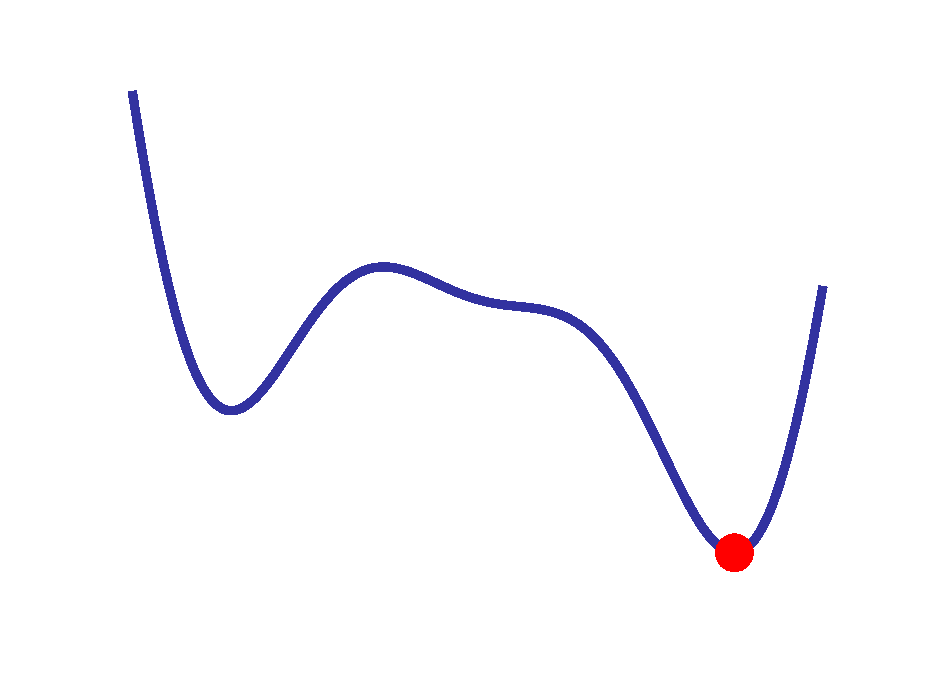
\includegraphics[width=.99\linewidth]{Pics/pretty_example_2.eps}}{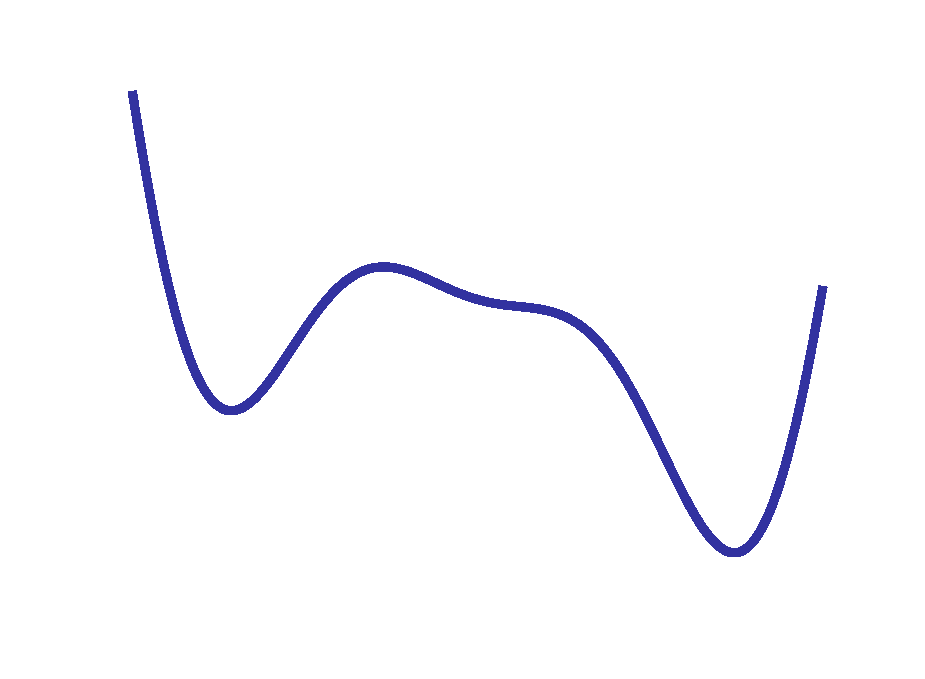
\includegraphics[width=.99\linewidth]{Pics/pretty_example_1.eps}}
\end{center}
\end{minipage}}\\
& \\[1.7cm]
\multicolumn{2}{l}{
\uncover<1->{\hspace{.15cm}\begin{minipage}{\linewidth}
 Numerous applications for modeling (physics, economics), estimation\newline{}(statistics, machine learning), decisions (control, operations research).}
\end{minipage}}\\[.3cm] 
\end{tabular}
\end{flushleft}

\end{frame}


\begin{frame}
\vspace{.2cm}
\small

\uncover<1->{Usually solved via {\bf iterative algorithm} generating sequence $x_0,x_1,\ldots,x_N$.}

\vspace{0.2cm}

\begin{center}
\begin{tabular}{@{}m{0.48\linewidth}@{}m{0.48\linewidth}@{}} % m{} for top alignment
% --- Image column ---
\uncover<1->{
      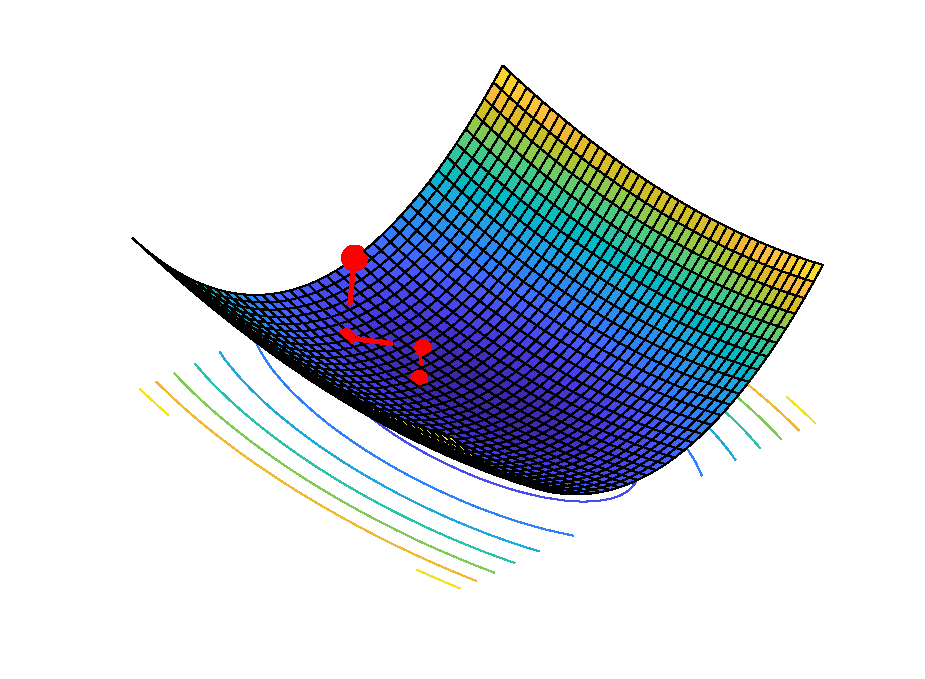
\includegraphics[width=\linewidth]{Pics/gradient_example3.eps}
}%
&\hspace{1cm}
% --- Algorithm column ---
\uncover<1->{%
\begin{minipage}[t]{\linewidth}\vspace{-2cm}
\scriptsize
\alt<3->{\vspace{-.5cm}
\newcommand{\ssu}{3}
\newcommand{\ssd}{4}
\newcommand{\sst}{5}
\newcommand{\ssq}{6}
\newcommand{\ssc}{7}	
\begin{tikzpicture}[scale=.7, transform shape]
				\begin{loglogaxis}[plotOptionsNeutral, ytick=\empty, xtick=\empty,ymin=1e-5, ymax=10,xmin=0,xmax=200,width=.99\linewidth,ylabel style={yshift=4pt,font=\small},xlabel style={yshift=-4pt,font=\small}]			
				\only<{\ssq}->{\addplot[color=mycolorThree,domain=1:100, samples=15,mark=*]{1/x^(2)}};
				\only<{\sst}->{\addplot[color=mycolorTwo,domain=1:55, samples=15,mark=*]{exp(-x/5)/exp(-1/5)}};%, only marks
				\only<{\ssu}->{\addplot[color=mycolorOne,domain=1:100, samples=15, mark=*]{exp(6.5/x)/exp(6.5)}
				};
				\only<{\ssc}->{\addplot[color=mycolorFour,domain=1:100, samples=15, mark=*]{(x/10+1/x^(2))/(1/10+1)}};
				\end{loglogaxis}
				\node[color=mycolorOne] (b1) at (1.4,2.4) {};
				\node[color=mycolorTwo] (b2) at (1.2,3.7) {};
				\node[color=mycolorThree] (b3) at (2.5,2.3) {};
				\node[color=mycolorFour] (b4) at (3,3.9) {};
				
				
				\node[color=mycolorOne] (a1) at (.5,-.9) {\alt<{\ssd}->{Fast, then stall?}{\color{white}Fast, then stall?}};
				\node[color=mycolorTwo] (a2) at (0.5,5) {\alt<{\sst}->{Slow, then fast?}{\color{white}Slow, then fast?}};
				\node[color=mycolorThree] (a3) at (5.5,2.6) {\alt<{\ssq}->{Smoothly improving?}{\color{white}Smoothly improving?}};
				\node[color=mycolorFour] (a4) at (5.8,4.8) {\alt<{\ssc}->{Diverging?}{\color{white}Diverging?}};
				\path[->, very thick, mycolorOne!60]<{\ssd}-> (a1.north) edge [out=90, bend left] (b1);
				\path[->, very thick, mycolorTwo!60]<{\sst}-> (a2.south) edge [ ] (b2);
				\path[->, very thick, mycolorThree!60]<{\ssq}-> (a3.west) edge  [out=90, bend right, in=200] (b3);
				\path[->, very thick, mycolorFour!60]<{\ssc}-> (a4.west) edge  [ bend right, in=250] (b4);
				\end{tikzpicture}}{\begin{tcolorbox}[width=.8\linewidth,colback=gray!20,boxsep=-1mm, arc=2mm,top=2.5mm,bottom=2.3mm,colframe=gray!20]\textbf{Gradient descent} (stepsize $\alpha$)\\[-0.2cm]
\begin{algorithmic}[]
\For{$k = 0, 1, \ldots$}\\
    \State $x_{k+1} = x_k - \alpha \nabla f(x_k)$\\
\EndFor
\end{algorithmic}
\end{tcolorbox}}
\end{minipage}
}%
\end{tabular}
\end{center}

\vspace{0.3cm}

\uncover<2->{What to expect from the output of the algorithm?}

\vspace{0.1cm}

\uncover<2->{For instance: \textbf{bounds} on certain notions of ``error'': $f(x_k)-f(x_\star)$, $\|x_k - x_\star\|$, $\|\nabla f(x_k)\|$, etc.}

\end{frame}


\frame{
\begin{center}
	{\Large{}How to show that an algorithm works?}\pause\\
	\vspace{1cm}
	{\begin{minipage}{.63\linewidth}\small
	\begin{itemize}
		\item<2-> Assumptions (no free lunch).
		\item<3-> Here: worst-case perspective.
	\end{itemize}
\end{minipage}
\begin{minipage}{.35\linewidth}
		\begin{tikzpicture}
    % Define the central formula
    \uncover<4>{\node (img) at (0,0) {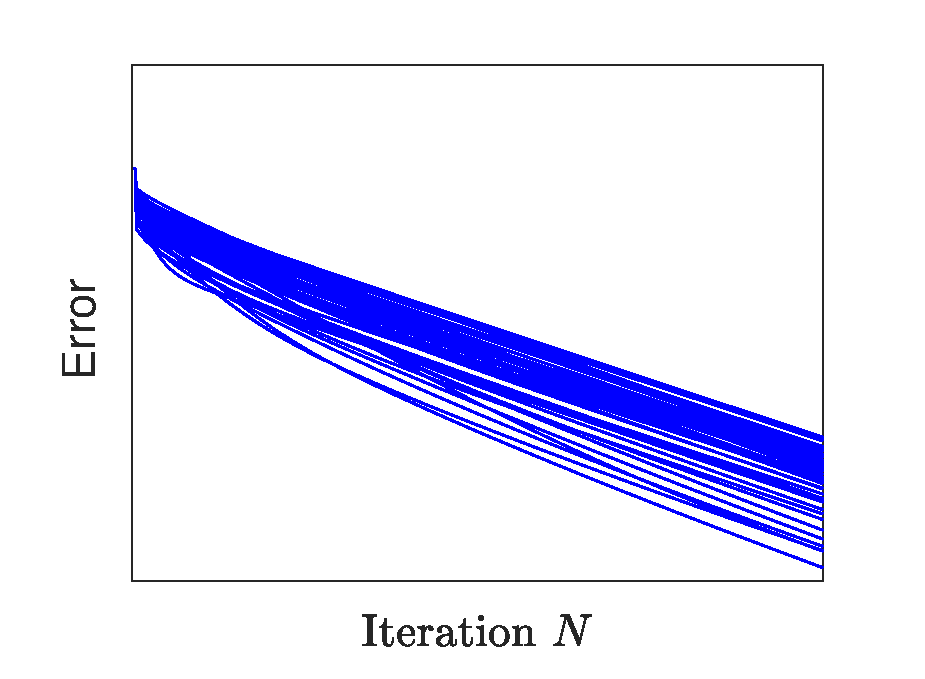
\includegraphics[height=.78\linewidth,width=.99\linewidth]{Pics/quads_GD_colors1.eps}};}
    \uncover<5->{\node (img) at (0,0) {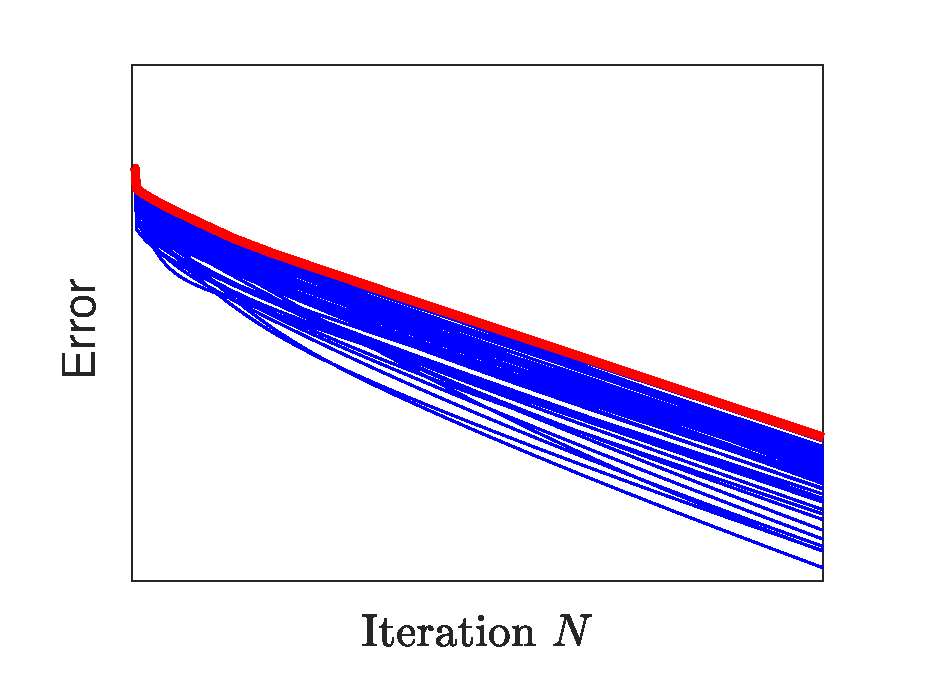
\includegraphics[height=.78\linewidth,width=.99\linewidth]{Pics/quads_GD_colors2.eps}};}
    \uncover<6->{\node (img) at (0,0) {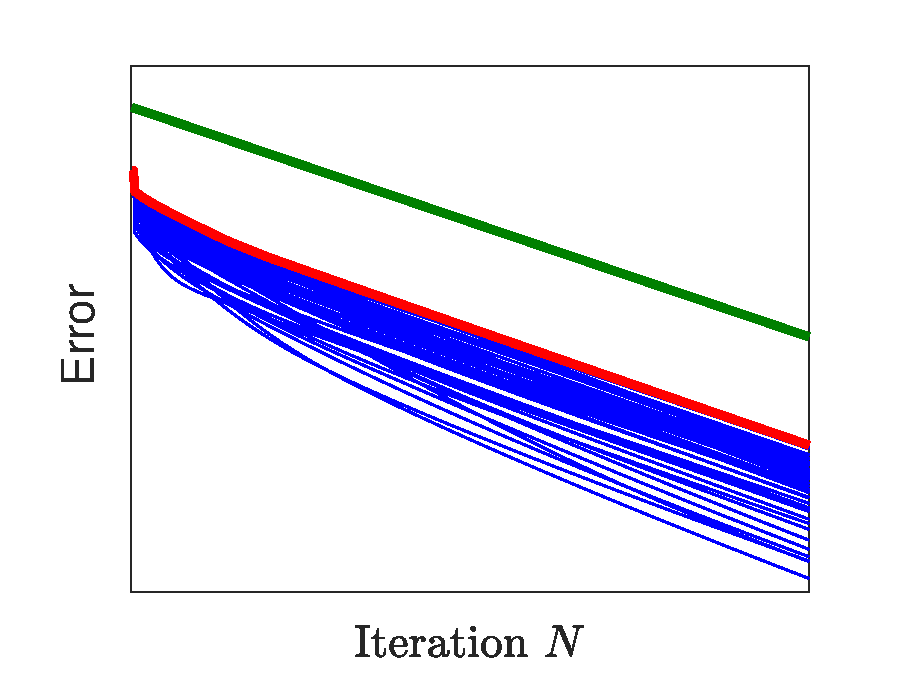
\includegraphics[height=.78\linewidth,width=.99\linewidth]{Pics/quads_GD_colors3.eps}};}
    \uncover<6->{\node [rotate=-20](uu) at (.55,.8) {{\color{darkgreen}upper bound}};}
    \uncover<5->{\node[rotate=-20] (tt) at (0,.4) {\color{red}\text{exact  certificate}};}
    \uncover<4->{\node[rotate=-20] (uu) at (0,-.7) {{\color{someBlue}errors} };}
\end{tikzpicture}
\end{minipage}}
\end{center}	
}

		

\begin{frame}
	\Large
	\tableofcontents
\end{frame}
\section{Constructive approach to performance analysis}
\begin{frame}
	\Large
	\tableofcontents [currentsection, hideothersubsections]
\end{frame}

\frame{
	\frtitle{Example: analysis of a gradient method }\small
	Let $f:\mathbb{R}^d\rightarrow \mathbb{R}$ (continuously differentiable). Find $x_\star\in\mathbb{R}^d$ such that \begin{align*}f(x_\star)=\min_{x\in \mathbb{R}^d} f(x),\end{align*}
	with $f$ is $L$-smooth and $\mu$-strongly convex ($f\in\mathcal{F}_{\mu,L}$).\\[.6cm]


	\uncover<2->{({Gradient method}) We decide to use: $x_{k+1}=x_k-\alpha  \nabla f(x_k)$}\\[.6cm]
	
	\uncover<3->{{\bf Question}: what \emph{a priori} guarantees after $N$ iterations?}\\[0.3cm]	\begin{itemize}
		\item<3->[]Examples: what about $f(x_N)-f(x_\star)$, $\norm{\nabla  f(x_N)}$, $\norm{x_N-x_\star}$?\\[.6cm]\end{itemize}
	
	
}


\frame{\frtitle{About the assumptions}\small
A differentiable function $f:\mathbb{R}^d\rightarrow \mathbb{R}$ is $\mu$-strongly convex and $L$-smooth iff $\forall x,y\in \mathbb{R}^d$:

\uncover<2->{\begin{center}
				\begin{tikzpicture}[yscale=0.35,xscale=0.35]
				\draw[very thick, black, -stealth] (-10.5,-0.1) -- (11.2,-0.1);
				\draw (11.2,-0.1) node[below left]{$x$};
				\draw[very thick, black, -stealth] (-10,-0.5) -- (-10,8);
				\draw (-10.1,8) node[left]{$f$};
				\draw(0,0) [very thick, color=blue, domain=-3*3:3*3, samples=50] plot({\x}, {2+(\x/4)^2});
				\uncover<3>{\draw(0,0) [dashed,very thick, color=red, domain=-8:0, samples=50] plot({\x}, {2+1-1/2*(\x+4)});}
				\uncover<4->{\draw(0,0) [dashed,very thick, color=red, domain=-8:0, samples=50] plot({\x}, {2+1-1/2*(\x+4)+((\x+4)/5)^2});}
				\uncover<5->{\draw(0,0) [dashed,very thick, color=red, domain=-6.5:-0.7, samples=50] plot({\x}, {2+1-1/2*(\x+4)+1/2*(\x+4)^2});}
				\node [color=red] (poi) at (-4,3) {$\bullet$};
				\end{tikzpicture}
			\end{center}}
			\begin{itemize}
				\item<3->[(1)] (Convexity) $f(x)\geqslant f(y) + \inner{ \nabla f(y)}{x-y}$, \\[0.3cm]
				\item<4->[(1b)] ($\mu$-strong convexity) $f(x) \geqslant f(y) + \inner{ \nabla f(y)}{x-y} +\frac{\mu}{2}\norm{x-y}^2$,\\[0.3cm]
				\item<5->[(2)] (L-smoothness) $f(x) \leqslant f(y) + \inner{\nabla f(y)}{x-y} +\frac{L}{2}\norm{x-y}^2$,\\[0.3cm]
				\item<6->[(1\&{}2)] $\langle{\nabla f(x)-\nabla f(y)};{x-y}\rangle  \geqslant        \tfrac{1}{L+\mu} \lVert{\nabla f(x)-\nabla f(y)}\rVert^2+\tfrac{\mu  L}{L+\mu}\lVert{x-y}\rVert^2$.
				
			\end{itemize}
		}
		
%\frame{assumptions}


%\frame{	\frtitle{Worst-case guarantee for gradient descent?}\scriptsize
%	
%	
%	
%	(Gradient method) For which $C(N,L)$ is
%	\[ f(x_N)-f_\star \leq C(N,L)\,\,{\|x_0-x_\star\|^2}\]
%	true for all $L$-smooth convex $f$ and $x_0\in\mathbb{R}^d$?
%	
%	{Find the worst possible function:
%		\uncover<2->{\begin{align*}
%			C(N,L)=\max_{f,x_0} \ &\frac{ f(x_N)-f_\star}{\|x_0-x_\star\|^2}\\[0.2cm]
%			\text{subject to: } & f \text{ satisfies some assumptions}  & \text{Problem class}\\[0.1cm]
%			&\uncover<2->{x_{k+1}=x_k-\gamma_k \nabla f(x_k) &\text{Algorithm}}\\[0.1cm]
%			\end{align*}}\uncover<3->{Such problem are infinite dimensional (function as a variable).\\[.5cm]}
%	}
%}

%%\frame{\frtitle{Smooth strongly convex functions}
%%	\small {Differentiable function $f:\mathbb{R}^d\rightarrow\mathbb{R}$, $f$ is ($\mu$-strongly) convex and $L$-smooth iff $\forall x,y\in \mathbb{R}^d$ we have:\\[0.3cm]
%%		
%%		\uncover<2->{\begin{center}
%%				\begin{tikzpicture}[yscale=0.35,xscale=0.35]
%%				\draw[very thick, black, -stealth] (-10.5,-0.1) -- (11.2,-0.1);
%%				\draw (11.2,-0.1) node[below left]{$x$};
%%				\draw[very thick, black, -stealth] (-10,-0.5) -- (-10,8);
%%				\draw (-10.1,8) node[left]{$f$};
%%				\draw(0,0) [very thick, color=blue!50, domain=-3*3:3*3, samples=50] plot({\x}, {2+(\x/4)^2});
%%%				\uncover<3>{\draw(0,0) [dashed,very thick, color=red, domain=-8:0, samples=50] plot({\x}, {2+1-1/2*(\x+4)});}
%%				\uncover<3->{\draw(0,0) [dashed,very thick, color=red, domain=-8:0, samples=50] plot({\x}, {2+1-1/2*(\x+4)+((\x+4)/5)^2});}
%%				\uncover<4->{\draw(0,0) [dashed,very thick, color=darkspringgreen, domain=-6.5:-0.7, samples=50] plot({\x}, {2+1-1/2*(\x+4)+1/2*(\x+4)^2});}
%%				\node [color=blue] (poi) at (-4,3) {$\bullet$};
%%				\end{tikzpicture}
%%		\end{center}}
%%		
%%		\begin{itemize}
%%			\item<3->[(1)] \textcolor{red}{($\mu$-strong convexity) $f(x) \geqslant f(y) + \inner{ \nabla f (y)}{x-y} +\frac{\mu}{2}\norm{x-y}^2$,}
%%			\item<4->[(2)] \textcolor{darkspringgreen}{(L-smoothness) $f(x) \leqslant f(y) + \inner{\nabla f (y)}{x-y} +\frac{L}{2}\norm{x-y}^2$.}
%%			
%%		\end{itemize}
%%	}
%%	
%%}


\frame{\frtitle{Convergence rate of a gradient step}\scriptsize
	\vspace{.1cm}
	\uncover<2->{\begin{center}\Ovalbox{ \begin{minipage}{.8\linewidth}\vspace{.3cm}{\bf Toy example}: What is the smallest $\tau$ such that:
					\[ \|x_1-x_\star \|^2 \leqslant \tau \|x_0-x_\star\|^2,\]
					for all
					\begin{itemize}
						\item<3-> $d\in\mathbb{N}$, $L$-smooth and $\mu$-strongly convex function $f$ (notation $f\in\mathcal{F}_{\mu,L}$),
						\item<4-> $x_0$, and $x_1$ generated by gradient step $x_1=x_0-\alpha \nabla f (x_0)$,
						\item<5-> $x_\star=\argmin{x} f(x)$?
	\end{itemize}\end{minipage} }\end{center} }\vspace{.1cm}
	\uncover<6->{
	\begin{equation*}
		\begin{aligned}
		\uncover<6->{\|x_{1}-x_\star\|^2}&\uncover<7->{=\|x_0-x_\star\|^2-2\alpha\langle \nabla f(x_{0});\,x_{0}-x_\star\rangle+\alpha^2\|\nabla f(x_{0})\|^2} \\
		&\uncover<8->{\,\Bigg\downarrow \text{ Inequality (1\&{}2)}} \\
		&\uncover<9->{\leq  \left(1-\tfrac{2\alpha L \mu}{L+\mu}\right)\lVert{x_0-x_\star}\rVert^2+\alpha\left(\alpha-\tfrac2{L+\mu}\right)\lVert{\nabla f(x_0)}\rVert^2}\\
		&\uncover<10->{\,\Bigg\downarrow \text{ if } 0\leq \alpha\leq \tfrac{2}{L+\mu}}\\
		&\uncover<11->{\leq (1-\alpha\mu)^2\|x_0-x_\star\|^2.}
		\end{aligned}
	\end{equation*}}
}

\frame{\frtitle{Convergence rate of a gradient step}\scriptsize
\begin{center}
{\begin{minipage}{.8\linewidth}\small
Legitimate questions:
	\begin{itemize}
		\item<2-> anything improvable? Realistic analyses?
		\item<3-> How to choose the right inequalities to combine? 
		\item<4-> Why studying this specific quantity? Possible to adapt to other quantities?
		\item<5-> Unique way to arrive to the desired result? 
		\item<6-> How likely are we to find such proofs in more complicated cases?
	\end{itemize}
\end{minipage}}
\end{center}
}

\frame{\frtitle{Legitimate questions about performance analyses?}\vspace{-1cm}
\begin{center}
\begin{tabular}{cc}
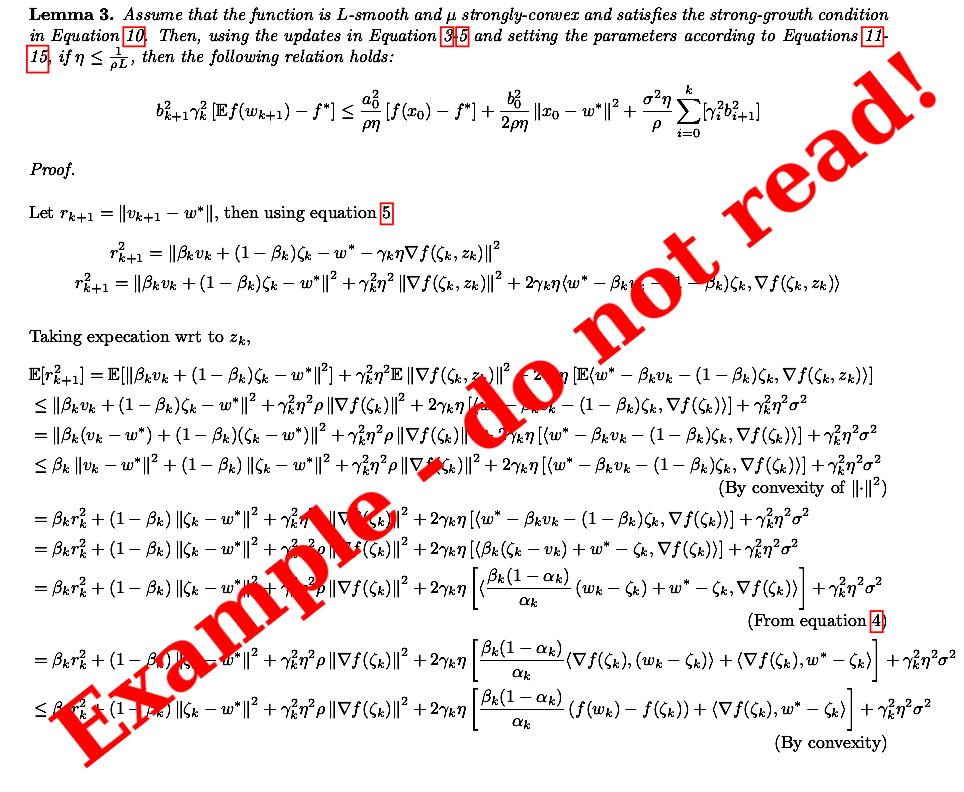
\includegraphics[height=.3\linewidth]{Pics/P1_V4.png} &{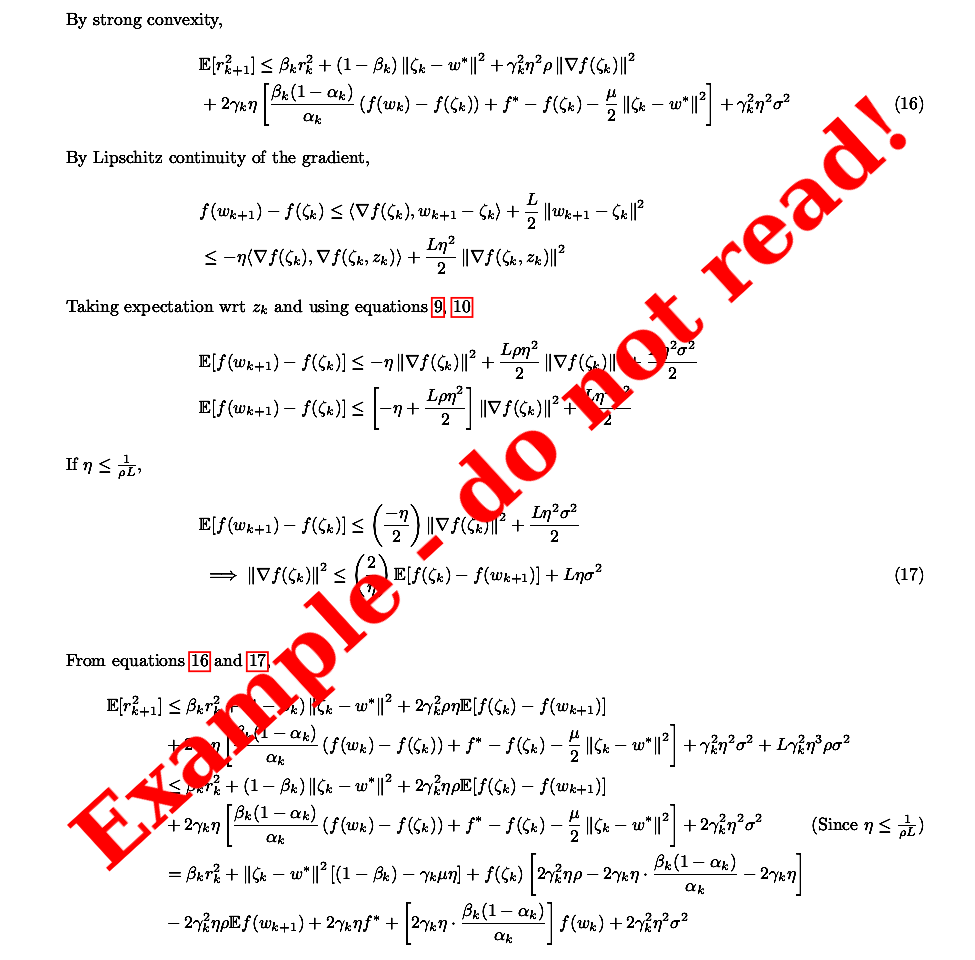
\includegraphics[height=.35\linewidth]{Pics/P2_V3.png}}\\
\end{tabular}
\end{center}
\vspace{-.2cm}
\uncover<2->{
\begin{tcolorbox}[colback=gray!20,width=1.0\textwidth,  arc=2mm,top=.5mm,bottom=.5mm,right=.5mm,left=-.5mm, colframe=gray!20] \normalsize
\begin{tabular}{ll}
\uncover<2->{{\textcolor{red}{\faWarning}} {Error-prone}} & \uncover<2->{{\textcolor{red}{\faQuestionCircleO}} Easily fixable?} \\
\uncover<2->{{\textcolor{red}{\faWarning}} {Technical}, {lack global insights.}} & \uncover<2->{{\textcolor{red}{\faQuestionCircleO}} Simple to adapt to variations of target inequality?} \\
\uncover<2->{{\textcolor{red}{\faWarning}} Few proof patterns.} & \uncover<2->{{\textcolor{red}{\faQuestionCircleO}} Simple to adapt to algorithmic variations?}\\ 
\end{tabular}
\end{tcolorbox}}
\vspace{-2.5cm}

}


\frame{\frtitle{Convergence rate of a gradient step}\scriptsize
	\vspace{.1cm}
	\uncover<2->{\begin{center}\Ovalbox{ \begin{minipage}{.8\linewidth}\vspace{.3cm}{\bf Toy example}: What is the smallest $\tau$ such that:
					\[ \|x_1-x_\star \|^2 \leqslant \tau \|x_0-x_\star\|^2,\]
					for all
					\begin{itemize}
						\item<2-> $d\in\mathbb{N}$, $L$-smooth and $\mu$-strongly convex function $f$ (notation $f\in\mathcal{F}_{\mu,L}$),
						\item<2-> $x_0$, and $x_1$ generated by gradient step $x_1=x_0-\alpha \nabla f (x_0)$,
						\item<2-> $x_\star=\argmin{x} f(x)$?
	\end{itemize}\end{minipage} }\end{center} }
	\begin{minipage}{.2\linewidth}
	\uncover<3->{Computing $\tau$?\footnotemark}\\[.3cm]
	
	\uncover<6->{\underline{Variables}: $f$, $x_0$, $x_1$, $x_\star$. \\[.1cm]}\uncover<6->{\underline{Parameters}: $\mu$, $L$, $\alpha$.} 
	\end{minipage}
	\begin{minipage}{.79\linewidth}
	\uncover<4->{
		\begin{align*}
		\tau= \max_{f,x_0,x_1,x_\star} \ &\frac{\|x_1-x_\star\|^2}{\|x_0-x_\star\|^2}\\[0.1cm]
		\text{s.t. } & f\in\mathcal{F}_{\mu,L}  &\text{Functional class}\\[0.1cm]
		&\uncover<5->{x_{1}=x_0-\alpha \nabla f (x_0) &\text{Algorithm}}\\[0.1cm]
		&\uncover<5->{\nabla f (x_\star)=0 &\text{Optimality of $x_\star$}}
		\end{align*}}
	\end{minipage}{\footnotetext[1]<3->{Original idea from [Drori and Teboulle, 2014]. Developments here from [T, Hendrickx, Glineur, 2017].}}
}
%\frame{\frtitle{Bibliographical references}	\scriptsize
%
%Important references:
%\begin{itemize}
%	\item . ``Performance of first-order methods for smooth convex minimization: a novel approach.'' Mathematical Programming 145 (1), 451-482.
%	\item Lessard, Recht, and Packard (2016). ``Analysis and design of optimization algorithms via integral quadratic constraints.'' SIAM Journal on Optimization 26 (1), 57-95.
%\end{itemize}
%Example follows the presentation lines from
%\begin{itemize}
%	\item T., Hendrickx, Glineur (2017). ``Smooth strongly convex interpolation and exact worst-case performance of first-order methods.'' Mathematical Programming 161, 307-345.
%\end{itemize}
%}


%%\pause
%%	{First part of the presentation:
%%	\begin{itemize}
%%		\item T., Hendrickx, Glineur ('17). ``Smooth strongly convex interpolation and exact worst-case performance of first-order methods.''
%%		\item T., Hendrickx, Glineur ('17). ``Exact worst-case performance of first-order methods for composite convex optimization.''
%%		\item T., Hendrickx, Glineur ('17). ``Performance estimation toolbox (PESTO): Automated worst-case analysis of first-order optimization methods.''
%%		\item Goujaud, Moucer, et al. ('22). ``PEPit: computer-assisted worst-case analyses of first-order optimization methods in Python.''
%%	\end{itemize}\pause
%%	Second part
%%	\begin{itemize}
%%		\item Drori, T ('20). ``Efficient first-order methods for convex minimization: a constructive approach.''
%%		\item Drori, T ('22). ``On the oracle complexity of smooth strongly convex minimization.''
%%		\item T, Drori ('23). ``An optimal gradient method for smooth strongly convex minimization.''
%%	\end{itemize}}
%%	\textbf{Informal introduction: \url{https://francisbach.com/computer-aided-analyses/}}.


\frame{\frtitle{Sampled version}\small	
	\begin{itemize}[leftmargin=*]
		\item<2-> Performance estimation problem \uncover<3->{\hfill{\bf ({Variables}: $f$, $x_0$, $x_1$, $x_\star$)}}:
		\begin{equation*}
		\begin{aligned}
		\maxim{\substack{f,x_0,x_1,x_\star}} \quad & \frac{{\|x_1-x_\star\|}^2}{\|x_0-x_\star\|^2}\\
		\text{subject to } \quad & \text{\color{red}$f$ is $L$-smooth and $\mu$-strongly convex,}\\
		& x_{1}=x_0-\alpha \nabla f (x_0)\\
		& \nabla f (x_\star)=0.
		\end{aligned}
		\end{equation*}
		\item<4-> Sampled version:  \uncover<6->{\hfill{\bf ({Variables}: $x_0$, $x_1$, $x_\star$, $g_0$, $g_\star$, $f_0$, $f_\star$)}}
		\uncover<5->{\begin{equation*}
			\begin{aligned}
			\maxim{\substack{x_0,x_1,x_\star\\g_0,g_\star\\f_0,f_\star}} \quad & \frac{{\|x_1-x_\star\|}^2}{\|x_0-x_\star\|^2}\\
			\text{subject to } \quad & {\color{red}\exists f\in\mathcal{F}_{\mu,L} \text{ such that }\left\{\begin{array}{ll}
				f_i=f(x_i)\quad & i=0,\star\\
				g_i=\nabla f (x_i)\quad & i=0,\star
				\end{array}\right.}\\
			& x_{1}=x_0-\alpha g_0\\
			& g_\star=0.\\
			\end{aligned}
			\end{equation*}}
	\end{itemize}
	
}

\frame{
	\frtitle{Smooth strongly convex interpolation (or extension)}\vspace{.2cm}
	\small
	Let $I$ index set, and associated $\left\{(x_i,g_i,f_i) \right\}_{i\in I}$: points $x_i$, (sub)gradients $g_i$ and function values~$f_i$.
	\uncover<2->{
		\begin{center}
			\begin{tikzpicture}[yscale=0.31,xscale=0.31]
			\tikzset{fleche/.style={->, >=latex, thick},
				flecheB/.style={<->, >=latex, very thick},
				droite/.style={thick,blue}};
			\draw[very thick, black, -stealth] (-10.5,-0.1) -- (11.2,-0.1);
			\draw (11.2,-0.1) node[below left]{$x$};
			\draw[very thick, black, -stealth] (-10,-0.5) -- (-10,8);
			\draw (-10.1,8) node[left]{$f$};
			\node [color=red] (point1) at (-8.5,6.51) {$\bullet$};
			\draw (point1.center) node[color=red,below left] {$x_0$};
			\draw(0,0) [very thick, color=red, domain=-9.1:-7.9, samples=2] plot({\x}, {6.51-1.06*(\x+8.5)});
			\node [color=red] (point2) at (7.3,5.33) {$\bullet$};
			\draw (point2.center) node[color=red,below right] {$x_2$};
			\draw(0,0) [very thick, color=red, domain=6.7:7.9, samples=2] plot({\x}, {5.33+0.91*(\x-7.3)});
			\node [color=red] (point3) at (-0.5,2) {$\bullet$};
			\draw (point3.center) node[color=red,below] {$x_1$};
			\draw(0,0) [very thick, color=red, domain=-1.3:0.3, samples=2] plot({\x}, {2+0.2*(\x+0.5)});
			\end{tikzpicture}
	\end{center}}
	\begin{itemize}[leftmargin=*]
		\item<2->[?] Possible to find $f\in\mathcal{F}_{\mu,L}$ such that $f(x_i)=f_i$, and $g_i=\nabla f(x_i)$ $\forall i\in I$?
		\item<3->[-] Necessary and sufficient condition: $\forall i,j\in I$ 
		\begin{align*}
		f_i\geqslant f_j+\inner{g_j}{x_i-x_{j}}+\tfrac{1}{2L}\normsq{g_i-g_j}+\tfrac{\mu}{2(1-\mu/L)}\normsq{x_i-x_j-\tfrac{1}{L}(g_i-g_j)}.
		\end{align*}
		\item<4->[-] Simpler example: pick $\mu=0$ and $L=\infty$ (just convexity):\[f_i\geqslant f_j+\inner{g_j}{x_i-x_{j}}.\]
	\end{itemize}
}

\frame{\frtitle{Replace constraints}\small
	
	\begin{itemize}[leftmargin=*]
		\item<2-> Interpolation conditions allow removing {\color{red}red} constraints 
		\begin{equation*}
		\begin{aligned}
		\maxim{\substack{x_0,x_1,x_\star\\g_0,g_\star\\f_0,f_\star}} \quad & \frac{{\|x_1-x_\star\|}^2}{\|x_0-x_\star\|^2}\\
		\text{subject to } \quad & {\color{red}\exists f\in\mathcal{F}_{\mu,L} \text{ such that }\left\{\begin{array}{ll}
			f_i=f(x_i)\quad & i=0,\star\\
			g_i=\nabla f (x_i)\quad & i=0,\star
			\end{array}\right.}\\
		& x_{1}=x_0-\alpha g_0\\
		&g_\star = 0,\\
		\end{aligned}
		\end{equation*}
		\item<3-> replacing them by{\color{red}
			\begin{equation*}
			\begin{aligned}
			f_\star\geqslant f_0+\inner{g_0}{x_\star-x_0}+\tfrac{1}{2L}\normsq{g_\star-g_0}+\tfrac{\mu}{2(1-\mu/L)}\normsq{x_\star-x_0-\tfrac{1}{L}(g_\star-g_0)}\\
			f_0\geqslant f_\star+\inner{g_\star}{x_0-x_\star}+\tfrac{1}{2L}\normsq{g_0-g_\star}+\tfrac{\mu}{2(1-\mu/L)}\normsq{x_0-x_\star-\tfrac{1}{L}(g_0-g_\star)}.
			\end{aligned}
			\end{equation*}}
		\item<4-> Same optimal value (no relaxation): {\color{red}non-convex quadratic} problem.
	\end{itemize}
	
}
%	\frame{\frtitle{Semidefinite lifting}\scriptsize
%		{\color{red}change to $\|x_1-x_\star\|^2$}
%		\begin{itemize}
%			\item<2-> Using $x_1=x_0-\gamma g_0$, all elements are quadratic in $(g_0,g_1)$, and linear in $(f_0,f_1)$:
%			\begin{equation*}
%			\begin{aligned}
%			\maxim{\substack{g_0,g_1\\f_0,f_1}} \quad & {\|g_1\|}^2\\
%			\text{subject to } \quad & f_1\geqslant f_0-\gamma\normsq{g_0}+\tfrac{1}{2L}\normsq{g_1-g_0}+\tfrac{\mu}{2(1-\mu/L)}\normsq{\gamma g_0+\tfrac{1}{L}(g_1-g_0)}\\
%			&f_0\geqslant f_1+\gamma\inner{g_1}{g_0}+\tfrac{1}{2L}\normsq{g_1-g_0}+\tfrac{\mu}{2(1-\mu/L)}\normsq{\gamma g_0+\tfrac{1}{L}(g_1-g_0)}\\
%			&\normsq{g_0}=R^2.
%			\end{aligned}
%			\end{equation*}
%			\item<3-> They are therefore {\color{red}linear} in terms of a Gram matrix $G$ and a vector $F$, with
%			\begin{align*}
%			G =  \begin{bmatrix}
%			\|g_0\|^2 & \langle g_0,g_1\rangle\\
%			\langle g_0, g_1\rangle & \| g_1\|^2
%			\end{bmatrix}=\begin{bmatrix}
%			g_0 & g_1
%			\end{bmatrix}^{\top\!}\begin{bmatrix}
%			g_0 & g_1
%			\end{bmatrix},\quad 	F = \begin{bmatrix}
%			f_0 & f_1
%			\end{bmatrix},
%			\end{align*}
%			where $G\succcurlyeq 0$ by construction.
%		\end{itemize}
%	}

\begin{frame}\frtitle{Semidefinite lifting}\small		
	\begin{itemize}[leftmargin=*]
		\item<1->Define $P\triangleq[x_0-x_\star,\, g_0]\in\mathbb{R}^{d\times 2}$ and $F \triangleq 			f_0-f_\star$.
		\item<2->Using new variables $G\succcurlyeq 0$ and $F$
		\begin{align*}
		G \triangleq P^TP= \begin{bmatrix}
		\|x_0-x_\star\|^2 & \langle g_0,x_0-x_\star\rangle\\
		\langle g_0, x_0-x_\star\rangle & \| g_0\|^2
		\end{bmatrix}\succcurlyeq 0,
		\end{align*}
		\item<3-> previous problem can be relaxed to $2\times 2$ SDP  
		\begin{equation*}
		\begin{aligned}
		\maxim{G,\, F} \quad & {G_{1,1}+\alpha^2 G_{2,2}-2\alpha G_{1,2}}\\
		\text{subject to } \quad & F + \tfrac{L\mu}{2(L-\mu)} G_{1,1}+\tfrac{1}{2(L-\mu)}G_{2,2}-\tfrac{L}{L-\mu}G_{1,2}\leqslant 0\\
		&-F + \tfrac{L\mu}{2(L-\mu)} G_{1,1}+\tfrac{1}{2(L-\mu)}G_{2,2}-\tfrac{\mu}{L-\mu}G_{1,2}\leqslant 0\\
		&{G_{1,1}= 1}\\
		&G\succcurlyeq 0
		\end{aligned}
		\end{equation*}
		\uncover<4->{(using homogeneity argument and substituting $x_1$ and $g_\star$).}
			\item<5-> Assuming $x_0,x_\star,g_0\in\real^d$ with $d\geqslant 2$, same optimal value as original problem!
			\item<6-> For $d=1$ same as original problem by adding $\rank(G)\leqslant 1$. 
			
		
	\end{itemize}
\end{frame}

\frame{\frtitle{Numerical solution of the SDP}\small
	Fix $L=1$, $\mu=.1$ and solve the SDP for a few values of $\alpha$.
	\uncover<2->{\begin{center}
			\begin{tikzpicture}
			\begin{axis}[legend pos=outer north east, legend style={draw=none},legend cell align={left},ylabel={$\frac{\|x_1-x_\star\|^2}{\|x_0-x_\star\|^2}$},xlabel={step-size $\alpha$}, plotOptions,  ymin=-.001, ymax=4,xmin=-1,xmax=3,width=.35\linewidth,ylabel style={rotate=-90}]
			\addplot [color=blue] table [x=stepsize,y=distance]  {Data/GM_rates.dat};
			\only<3->{\addplot [domain=-1:0, samples=50, very thick, red] { (1 - x)^2 };}
			\only<3->{\addplot [domain=2:3, samples=50, very thick, red] { (1- x)^2  };}
			\end{axis}
			\end{tikzpicture}
	\end{center}}
	\uncover<3->{Observations:}
	\begin{itemize}
		\item<3->{numerics match the known $\max\{(1-\alpha L)^2,(1-\alpha\mu)^2\}$}
		\item<3-> recovers that gradient descent converges for $\alpha\in (0,2/L)$ (\textcolor{red}{divergence otherwise}).
	\end{itemize}
}


	
		\begin{frame}\frtitle{Dual problem}\scriptsize
			
			\begin{itemize}
				\item<1-> Dual problem is
				{\begin{align*}
					\minim{\co{\tau},\co{\lambda_1},\co{\lambda_2}\geqslant 0} & \,\co{\tau}\\
					\text{subject to }& S=\begin{bmatrix}
					\co{\tau}-1+\frac{\co{\lambda_1} L\mu}{L-\mu } & {\alpha}-\frac{\co{\lambda_1} (L+\mu)}{2 (L-\mu )} \\
					{\alpha}-\frac{\co{\lambda_1} (L+\mu)}{2 (L-\mu )} & \frac{\co{\lambda_1}}{L-\mu }-{\alpha^2} \\
					\end{bmatrix}\succcurlyeq 0\\
					&0=\co{\lambda_1}-\co{\lambda_2}.
					\end{align*}
				}
				\item<2-> Weak duality:  any dual feasible point $\equiv$ valid worst-case convergence rate \uncover<4->{({${\color{blue}\Uparrow}$}).}
				\item<3-> Direct consequence: for any $\co{\tau}\geqslant 0$ we have
				\begin{center}\Ovalbox{\begin{minipage}{.85\linewidth}\begin{center}
								$\|x_1-x_\star\|^2\leq \co{\tau} \|x_0-x_\star\|^2$ for all $f\in\mathcal{F}_{\mu,L}$, all $x_0\in\mathbb{R}^d$, all $d\in\mathbb{N}$, with $x_1=x_0-{\alpha} \nabla f(x_0)$.\\[.1cm] {${\color{blue}\Big\Uparrow}$\hspace{.2cm}\uncover<6->{${\color{red}\Big\Downarrow}$}}\\[.1cm]$\exists\co{\lambda}\geq 0:\,\begin{bmatrix}
								\co{\tau}-1+\frac{ \co{\lambda} L\mu}{L-\mu }  & {\alpha}-\frac{\co{\lambda} (L+\mu)}{2 (L-\mu )} \\
								{\alpha}-\frac{\co{\lambda} (L+\mu)}{2 (L-\mu )} & \frac{\co{\lambda}}{L-\mu }-{\alpha^2} \\
								\end{bmatrix}\succcurlyeq 0$
							\end{center}
					\end{minipage}}\vspace{.3cm}
				\end{center}
				\item<5-> Strong duality holds  ($\exists$ Slater point): any valid worst-case convergence rate $\equiv$ valid dual feasible point ({${\color{red}\Downarrow}$}).
			\end{itemize}	
		\end{frame}


\frame{\frtitle{Dual solutions}\scriptsize
	Fix $L=1$, $\mu=.1$ and solve the dual SDP for a few values of $\alpha$.
	\uncover<2->{\begin{center}
			\begin{tikzpicture}
			\begin{axis}[legend pos=outer north east, legend style={draw=none},legend cell align={left},ylabel={Dual values ($\co{\lambda_1}$ and $\co{\lambda_2}$)},xlabel={Step size ${\alpha}$}, plotOptions,  ymin=-.001, ymax=12,xmin=-1,xmax=3,width=.35\linewidth]
			\addplot [color=red] table [x=stepsize,y=dist_dualval1]  {Data/GM_rates.dat};\addlegendentry{$\co{\lambda_1}$}
			\addplot [color=blue, dashed] table [x=stepsize,y=dist_dualval2]  {Data/GM_rates.dat};\addlegendentry{$\co{\lambda_2}$}
			\end{axis}
			\end{tikzpicture}
	\end{center}}
	\uncover<3->{Numerics match $\co{\lambda_1}=\co{\lambda_2}={2}{|{\alpha}|} \rho({\alpha})$ with $\rho({\alpha})=\max\{{\alpha} L-1,1-{\alpha}\mu\}$.}
}

			
		\frame{\frtitle{Recovering a ``standard'' proof}
		\scriptsize
		Gradient with ${\alpha}=\frac{1}{L}$. Perform weighted sum of two inequalities
		\uncover<2->{\begin{align*}
			&f_0\geqslant f_{\star}+\tfrac{1}{2L}\normsq{\nabla f(x_0)}+\tfrac{\mu}{2(1-\mu/L)}\normsq{x_0-x_{\star}-\tfrac{1}{L}\nabla f(x_0)} \quad &:\co{\lambda_1}\uncover<4->{{=2 {\alpha} (1- {\alpha}\mu)}}\\
			&
			f_{\star}\geqslant f_0+\inner{\nabla f(x_0)}{x_{\star}-x_0}+\tfrac{1}{2L}\normsq{\nabla f(x_0)} +\tfrac{\mu}{2(1-\mu/L)}\normsq{x_0-x_{\star}-\tfrac{1}{L}\nabla f(x_0)} 
			&:\co{\lambda_2}\uncover<4->{{=2 {\alpha} (1- {\alpha}\mu)}}
			\end{align*}}\uncover<3->{with {$\co{\lambda_1},\co{\lambda_2}\geqslant 0$}. Weighted sum can be \alert{reformulated} as}
		\uncover<5->{{\begin{align*}
				\lVert{x_{1}-x_\star}\rVert^2  \leqslant      & \left(1- {\alpha}\mu  \right)^2\lVert{x_{0}-x_\star}\rVert^2 -\underbrace{{\alpha}\tfrac{2-{\alpha} (L+\mu)}{L-\mu} \lVert{\mu {(x_0  -x_\star)} - \nabla f(x_0)}\rVert^2}_{\uncover<6->{\geqslant 0\uncover<9->{, \color{red} \text{ or $=0$ when worst-case is achieved}}}},\\
				\uncover<7->{\leqslant & \left(1- {\alpha}\mu \right)^2 	\lVert{x_{0}-x_\star}\rVert^2,}
				\end{align*}}}
		\uncover<8->{leading to $\norm{ x_1-x_\star}^ 2\leqslant \left(1- {\alpha}\mu  \right)^2\lVert{x_{0}-x_\star}\rVert^2$} \uncover<10->{{\color{red}(tight)}.}
	}
			
\begin{frame}\frtitle{What did we do, so far?}\small
	
Summary:
			\begin{itemize}
				\item<2-> we computed the smallest $\tau(\mu,L,{\alpha})$ such
				that 
				\[ \|x_1-x_\star\|^2 \leq\tau(\mu,L,{\alpha})\,\|x_0-x_\star\|^2 \]
				is satisfied for all $x_0\in\mathbb{R}^d$, $d\in\mathbb{N}$, $f\in\FmuL$, and $x_1=x_0-{\alpha} \nabla f(x_0)$.\\[.2cm]
				\item<3-> Feasible points to primal SDP correspond to lower bounds on $\tau(\mu,L,{\alpha})$.\\[.2cm]
				\item<4-> Feasible points to dual SDP correspond to upper bounds on $\tau(\mu,L,{\alpha})$.
				\begin{itemize}
					\item<5-> proof via linear combinations of interpolation inequalities (evaluated at $\{x_k\}_k$ and $x_\star$),
					\item<5-> proofs can be rewritten as a ``sum-of-squares'' certificates (sum of squared norms).\\[.4cm]
				\end{itemize}
			\end{itemize}

			\end{frame}

\frame{\frtitle{Back to legitimate questions}\scriptsize
\begin{center}
{\begin{minipage}{.8\linewidth}\small
Legitimate questions (gradient descent, one iteration):
	\begin{itemize}
		\item anything improvable? Realistic analyses?
		\item How to choose the right inequalities to combine? 
		\item Why studying this specific quantity? Possible to adapt to other quantities?
		\item Unique way to arrive to the desired result? 
		\item How likely are we to find such proofs in more complicated cases?
	\end{itemize}
\end{minipage}}
\end{center}
}
%%\frame{\frtitle{When does it work?}\small
%%	The methodology applies, as is, as soon as:
%%	\begin{itemize}
%%		\item<2-> performance measure and initial condition are linear in $G$ and $F$,
%%		\item<3-> interpolation inequalities are linear in $G$ and $F$,
%%		\item<4-> algorithm can be described linearly in $G$ and $F$,\\[.5cm]
%%	\end{itemize}
%%	\uncover<5->{(but other cases are not doomed).}
%%	
%%
%%}

\frame{\frtitle{Missing details (next)}\small

Details that we did not cover so far:
\begin{itemize}
	\item (convex) interpolation
	\item semidefinite programming,
	\item (Lagrange) duality.
\end{itemize}

When does the approach actually work?
\begin{itemize}
	\item Function classes?
	\item Families of algorithms?
	\item Types of guarantees?
\end{itemize}
}

%%
%%\begin{frame}\frtitle{Performance estimation \& gradient descent}\small
%%	
%%	\begin{itemize}[leftmargin=*]
%%		\item We can compute for the smallest $\tau(L,\mu,\alpha)$ such
%%		that 
%%		\[ \|x_1-x_\star\|^2 \leq\tau(L,\mu,\alpha)\|x_0-x_\star\|^2 \]
%%		is satisfied for all $x_0\in\mathbb{R}^d$, $d\in\mathbb{N}$, $f\in\mathcal{F}_{\mu,L}$, and $x_1=x_0-\alpha \nabla f(x_0)$.\\[.2cm]
%%		\item<2-> Feasible points to previous SDP $\rightarrow$ lower bounds on $\tau(L,\mu,\alpha)$.\\[.2cm]
%%		\item<3-> Feasible points to dual SDP $\rightarrow$ upper bounds on $\tau(L,\mu,\alpha)$.\\[.2cm]
%%		\item<4-> How general is this?
%%		\begin{itemize}
%%			\item[$\rightarrow$] A few examples next!
%%		\end{itemize}
%%		\item<5-> What can we learn on the analysis structures?
%%		\begin{itemize}
%%			\item[$\rightarrow$] \begin{minipage}{.88\linewidth}
%%			Goujaud, Dieuleveut, T (2023). ``On fundamental proof structures in first-order optimization.'' Conference on Decision and Control (CDC).
%%			\end{minipage}
%%			\begin{minipage}{.11\linewidth}
%%			 \includegraphics[width=.5\linewidth]{Pictures/Baptiste.jpeg}\includegraphics[width=.4\linewidth]{Pictures/Aymeric.jpeg}
%%			\end{minipage}\\[.25cm]
%%						\item[$\rightarrow$] In this formalism, ``performance analyses $\equiv$ dual feasible points''.
%%		\end{itemize}
%%%		\item<4-> Want to know more?
%%%		\begin{itemize}
%%%			\item \url{https://francisbach.com/computer-aided-analyses/}
%%%			\item Toolboxes (next slides).
%%%			\item Dictates structure of proofs! $\rightarrow$ Baptiste/Aymeric...\\[.2cm]
%%%		\end{itemize}
%%%		\item<5-> Next:
%%%		\begin{itemize}
%%%			\item<5-> {Examples: performance guarantees after $N$ iterations.}
%%%			\item<6-> Beyond horizon-dependent ($N$) bounds...
%%%		\end{itemize}
%%	\end{itemize}
%%\end{frame}


%\begin{frame}
%NEXT: what to put in an example notebook?
%\end{frame}


%%%\frame{\frtitle{Example 1: gradient methods and momentum}\small
%%%\[ \min_{x\in\mathbb{R}^d} f(x),\]
%%%with $f$ an $L$-smooth convex function.\pause{} Three algorithms:\pause{}
%%%\begin{itemize}
%%%	\item Gradient descent: $x_{k+1}=x_k-\tfrac1L\nabla f(x_k).$\pause{}
%%%	\item Heavy-ball method [Polyak, 1964] $x_{k+1} = x_k - \alpha \nabla f(x_k) + \beta (x_k - x_{k-1})$ \pause{}\\ {\scriptsize{}(choice: $\alpha = \tfrac{1}{2L}$, $\beta=\sqrt{1 - L\alpha}$, see [Ghadimi, Feyzmahdavian, Johansson, 2015])}\pause{}
%%%	\item Accelerated gradient method [Nesterov, 1983]:
%%%\begin{equation*}
%%%\begin{aligned}
%%%x_{k+1} &= y_k - \tfrac1L \nabla f(x_k)\\
%%%y_{k+1} &= x_{k+1}+\tfrac{k-1}{k+1}(x_{k+1} - x_{k}).
%%%\end{aligned}
%%%\end{equation*}
%%%\end{itemize}\pause{}
%%%What can we guarantee on...
%%%\[ \frac{f(x_N)-f(x_\star)}{\|x_0-x_\star\|^2}\leq ?\quad\quad \frac{\|\nabla f(x_N)\|^2}{\|x_0-x_\star\|^2}\leq ?\quad\quad \frac{\underset{{0\leq k\leq N}}{\min}\|\nabla f(x_k)\|^2}{\|x_0-x_\star\|^2}\leq ?\]
%%%
%%%
%%%}
%%%
%%%\frame{\frtitle{Example 2: a primal-dual proximal point}\small
%%%	\uncover<1->{Minimize sum of two convex (ccp) functions
%%%		\[ \min_{x\in\mathbb{R}^d} f(x)+h(x)\]
%%%	assume $\exists x_\star,y_\star$ (KKT point): $-y_\star\in\partial f(x_\star),\, x_\star\in\partial h^*(y_\star)$.\\[.1cm]
%%%	\uncover<2->{\begin{center}
%%%		\fbox{
%%%			\parbox{0.95\textwidth}{
%%%				\textbf{Primal-dual proximal point algorithm} (see, e.g.,~[Rockafellar, 1976])
%%%				\begin{itemize}[leftmargin=*]
%%%					\item[] Input: $f,h$ convex (ccp) functions, $(y_0,x_0)\in\mathbb{R}^d\times \mathbb{R}^d$.\\[-0.6cm]
%%%					\item[] For $k=0,1,\ldots$\\[-0.75cm]
%%%					\begin{align*}
%%%					(y_{k+1},x_{k+1})=&\underset{y\in\mathbb{R}^d}{\mathrm{argmax}}\,\,\underset{x\in\mathbb{R}^d}{\mathrm{argmin}} \Bigl\{f(x)-h^*(y)+\langle y,\, x\rangle  \\& \quad\quad\quad\quad\quad\quad\quad\quad\quad+\tfrac1{2\alpha} \normsq{x-x_k}-\tfrac1{2\alpha} \normsq{y-y_k} \Bigl\}\\[-.9cm]
%%%					\end{align*}
%%%				\end{itemize}
%%%		}}
%%%	\end{center}}
%%%	\vspace{.1cm}
%%%	\uncover<3->{What guarantees of type (for some elements of $\partial f$ and $\partial h^*$)
%%%	\[ \frac{\|\partial f(x_N)+y_N\|^2 + \|x_N-\partial h^*(y_N)\|^2}{\|x_0 - x_\star\|^2+\|y_0-y_\star\|^2}\leq \tau(N,\alpha)?\]
%%%%See \href{/home/ataylor/Github/Presentations/2024/HDR/Examples/PD_ProximalPoint.ipynb}{\textsc{PEPit}}.
%%%}
%%%	
%%%}
%%%}
%%%\frame{\frtitle{Recap'}
%%%	\small \uncover<1->{
%%%		\begin{itemize}
%%%			\item<2->[\color{cadmiumgreen} \bf \large \smiley] Worst-case guarantees \emph{cannot be improved}, systematic approach,
%%%			\item<2->[\color{cadmiumgreen} \bf \large \smiley] allows reaching analyses that could barely be obtained by hand,
%%%			\item<2->[\color{cadmiumgreen} \bf \large \smiley] fair amount of scenarios/algorithms (e.g., proximal terms, stochastic, etc.),
%%%			\item<2->[\color{red} \bf \large \frownie] SDPs typically become prohibitively large in a variety of scenarios,
%%%			\item<2->[\color{red} \bf \large \frownie] transient behavior VS.~asymptotic behavior: might be hard to distinguish with small $N$,
%%%			\item<2->[\color{red} \bf \large \frownie] {proofs} (may be) quite involved and hard to intuit,
%%%			\item<2->[\color{red} \bf \large \frownie] proofs (may be) hard to generalize.
%%%				\end{itemize}}
%%%			}

%%%\begin{frame}\frtitle{A few instructive examples}\scriptsize \vspace{.1cm}
%%%	Worst-case analysis for fixed-point iterations:
%%%	\begin{itemize}
%%%		\item Lieder (2021). ``On the convergence of the Halpern-iteration''. Optimization letters 15(2).
%%%	\end{itemize}
%%%	Analysis of the proximal-point algorithm for monotone inclusions:
%%%	\begin{itemize}
%%%		\item Gu, Yang (2019). ``Optimal nonergodic sublinear convergence rate of the proximal point algorithm for maximal monotone inclusion problems''. SIAM Journal on Optimization 30(3).
%%%	\end{itemize}
%%%	Application to nonconvex optimization:
%%%	\begin{itemize}
%%%		\item Abbaszadehpeivasti, de Klerk, Zamani (2022). ``The exact worst-case convergence rate of the gradient method with fixed step lengths for $L$-smooth functions''. Optimization Letters 16(6).
%%%	\end{itemize}
%%%	Applications to distributed optimization:
%%%	\begin{itemize}
%%%		\item Sundararajan, Van Scoy, Lessard (2020). ``Analysis and design of first-order distributed optimization algorithms over time-varying graphs.'' IEEE Transactions on Control of Network Systems 7(4).
%%%		\item Colla, Hendrickx (2023). ``Automatic performance estimation for decentralized optimization.''  IEEE Transactions on Automatic Control 68(12).
%%%	\end{itemize}
%%%	Gradient descent for smooth convex minimization (definitive answers):
%%%	\begin{itemize}
%%%		\item Teboulle, Vaisbourd (2023). ``An elementary approach to tight worst case complexity analysis of gradient based methods.'' Mathematical Programming 201(1).
%%%	\end{itemize}
%%%\end{frame}
%%%
%%%
%%%
%%%\begin{frame}\frtitle{A few references} \scriptsize
%%%Historical reference: \\[.1cm]
%%%\begin{tabular}{lll}
%%%	$\diamond$ & \multirow{2}{.75\linewidth}{Drori, Teboulle (2014). ``Performance of first-order methods for smooth convex minimization: a novel approach.'' Mathematical Programming 145 (1).} & {\begin{minipage}{0.18\linewidth}{
\includegraphics[height=.2\linewidth]{Pictures/Yoel.jpg}\includegraphics[height=.2\linewidth]{Pictures/marc.jpeg}}
%%%        \end{minipage}}\\
%%%	& & \\[.1cm]
%%%\end{tabular}
%%%
%%%Main messages of this part:\\[.05cm]
%%%\begin{tabular}{lll}
%%%	$\diamond$ & \multirow{2}{.75\linewidth}{T, Hendrickx, Glineur (2017). ``Smooth strongly convex interpolation and exact worst-case performance of first-order methods.'' Mathematical Programming 161.} & {\begin{minipage}{0.18\linewidth}{\includegraphics[height=.2\linewidth]{Pictures/Julien.jpg}\includegraphics[height=.2\linewidth]{Pictures/Francois.jpeg}}
%%%        \end{minipage}}\\
%%%	& & \\[.05cm]
%%%	$\diamond$ & \multirow{2}{.75\linewidth}{Goujaud, Dieuleveut, T (2023). ``On fundamental proof structures in first-order optimization.'' Conference on Decision and Control (CDC).} & {\begin{minipage}{0.18\linewidth}{\includegraphics[height=.2\linewidth]{Pictures/Baptiste.jpeg}\includegraphics[height=.2\linewidth]{Pictures/Aymeric.jpeg}}
%%%        \end{minipage}}\\
%%%	& & \\[.05cm]
%%%	$\diamond$ & \multirow{2}{.75\linewidth}{Goujaud, Moucer, Glineur, Hendrickx,  T, Dieuleveut (2024). ``\textsc{PEPit}: computer-assisted worst-case analyses of first-order optimization methods in Python.''
%%%Mathematical Programming Computation 16(3).} & {\begin{minipage}{0.18\linewidth}{\includegraphics[height=.2\linewidth]{Pictures/Baptiste.jpeg}\includegraphics[height=.2\linewidth]{Pictures/Celine.jpeg}\includegraphics[height=.2\linewidth]{Pictures/Julien.jpg}\includegraphics[height=.2\linewidth]{Pictures/Francois.jpeg}\includegraphics[height=.2\linewidth]{Pictures/Aymeric.jpeg}}
%%%        \end{minipage}}\\
%%%	& & \\[.5cm]
%%%\end{tabular}
%%%
%%%\uncover<2->{To go further:\\[.05cm]
%%%\begin{tabular}{lll}
%%%	$\diamond$ & \multirow{2}{.75\linewidth}{T, Hendrickx, Glineur (2017). ``Exact worst-case performance of first-order methods for composite convex optimization.'' SIAM Journal on Optimization 27(3).} & {\begin{minipage}{0.18\linewidth}{\includegraphics[height=.2\linewidth]{Pictures/Julien.jpg}\includegraphics[height=.2\linewidth]{Pictures/Francois.jpeg}}
%%%        \end{minipage}}\\
%%%	& & \\[.05cm]
%%%	$\diamond$ & \multirow{2}{.75\linewidth}{Dragomir, T, d'Aspremont, Bolte (2022). ``Optimal complexity and certification of Bregman first-order methods.'' Mathematical Programming 194.} & {\begin{minipage}{0.18\linewidth}{\includegraphics[height=.2\linewidth]{Pictures/Radu.jpeg}\includegraphics[height=.2\linewidth]{Pictures/alexandre_daspremont.jpeg}\includegraphics[height=.2\linewidth]{Pictures/Jerome.jpg}}
%%%        \end{minipage}}\\
%%%	& & \\[.1cm]
%%%	$\diamond$ & \multirow{2}{.75\linewidth}{Barr\'e, T, Bach (2023). ``Principled analyses and design of first-order methods with inexact proximal operators.'' Mathematical Programming 201(1).} & {\begin{minipage}{0.18\linewidth}{
\includegraphics[height=.2\linewidth]{Pictures/mathieu.jpeg}
\includegraphics[height=.2\linewidth]{Pictures/FrancisV2.jpeg}}
%%%        \end{minipage}}\\
%%%	& & \\[.1cm]
%%%\end{tabular}}
%%%
%%%
%%%\end{frame}
%%%



	




\end{document}


















